\chapter{Der QHScompiler} \label{cha:4-QHS_Compiler}
Der QHScompiler, wie in Kapitel \ref{cha:2-Vergleich} bereits angesprochen, basiert auf einem von mir erdachten alternativen Aufbau für einen Compiler. Diesem Aufbau liegt eine einfache Idee zugrunde:
Die Macros der \textit{Macro Expansion} aus Abschnitt \ref{sec:traditional_code_generation} sollen erst während der Kompilierung innerhalb der Eingabedatei und nicht im Compiler definiert werden. 
Auf dieser Grundidee werde ich zwei Dinge aufbauen. Erstens halte ich es für möglich, mit der richtigen Verwendung von Macros die gesamte syntaktische Analyse zu überspringen und keinen AST generieren zu müssen.
Zweitens sollte es rein durch die Veränderung von diesen Macros möglich sein jegliche Programmiersprache zu kompilieren. Man könnte also in einem Dokument verschiedene Programmiersprachen verwenden und
müsste dazwischen bloss die jeweiligen Macros neu definieren. Das gleiche gilt ebenfalls für die Ausgabesprache.
Nur durch das Umdefinieren der Macros liesse sich die Ausgabesprache wechseln, ohne eine Änderung am Compiler vornehmen zu müssen.
Um dies zu verwirklichen, unterscheidet sich der QHScompiler stark von traditionellen Compilern.
%Um dies zu verwirklichen, folgt mein alternativer Ansatz einem Aufbau, der sich stark von einem traditionellen Compiler unterscheidet.

Die Programmiersprache, in der sich diese Macros definieren lassen, bezeichne ich als QHS. Der Compiler der QHS versteht und kompiliert, wird dazu passend QHScompiler genannt.
QHS besteht wie die meisten anderen Programmiersprachen aus Wörtern. Im Kontext von QHS werden diese Wörter \textit{Orders} genannt.
Orders können drei verschiedenen Typen aufweisen: \textit{Identifiers}, \textit{Instructions} und \textit{LiteralCode}.
%Bei \textit{Identifiers} handelt es sich um die bereits erwähnten Macros, \textit{Instructions} sind einfache vorprogrammierte Anweisungen an den QHScompiler und \textit{LiteralCode} ist Text, der unverändert in die Ausgabedatei geschrieben wird.
Wie diese drei \textit{Ordertypen} genau funktionieren, wird in Abschnitt \ref{sec:qhs-execute} ausführlicher erklärt.

Der Kompilierung durch den QHScompiler liegt ein einfacher Zyklus, der QHS-Zyklus, zugrunde.

\begin{figure}[h!]
    \centering
    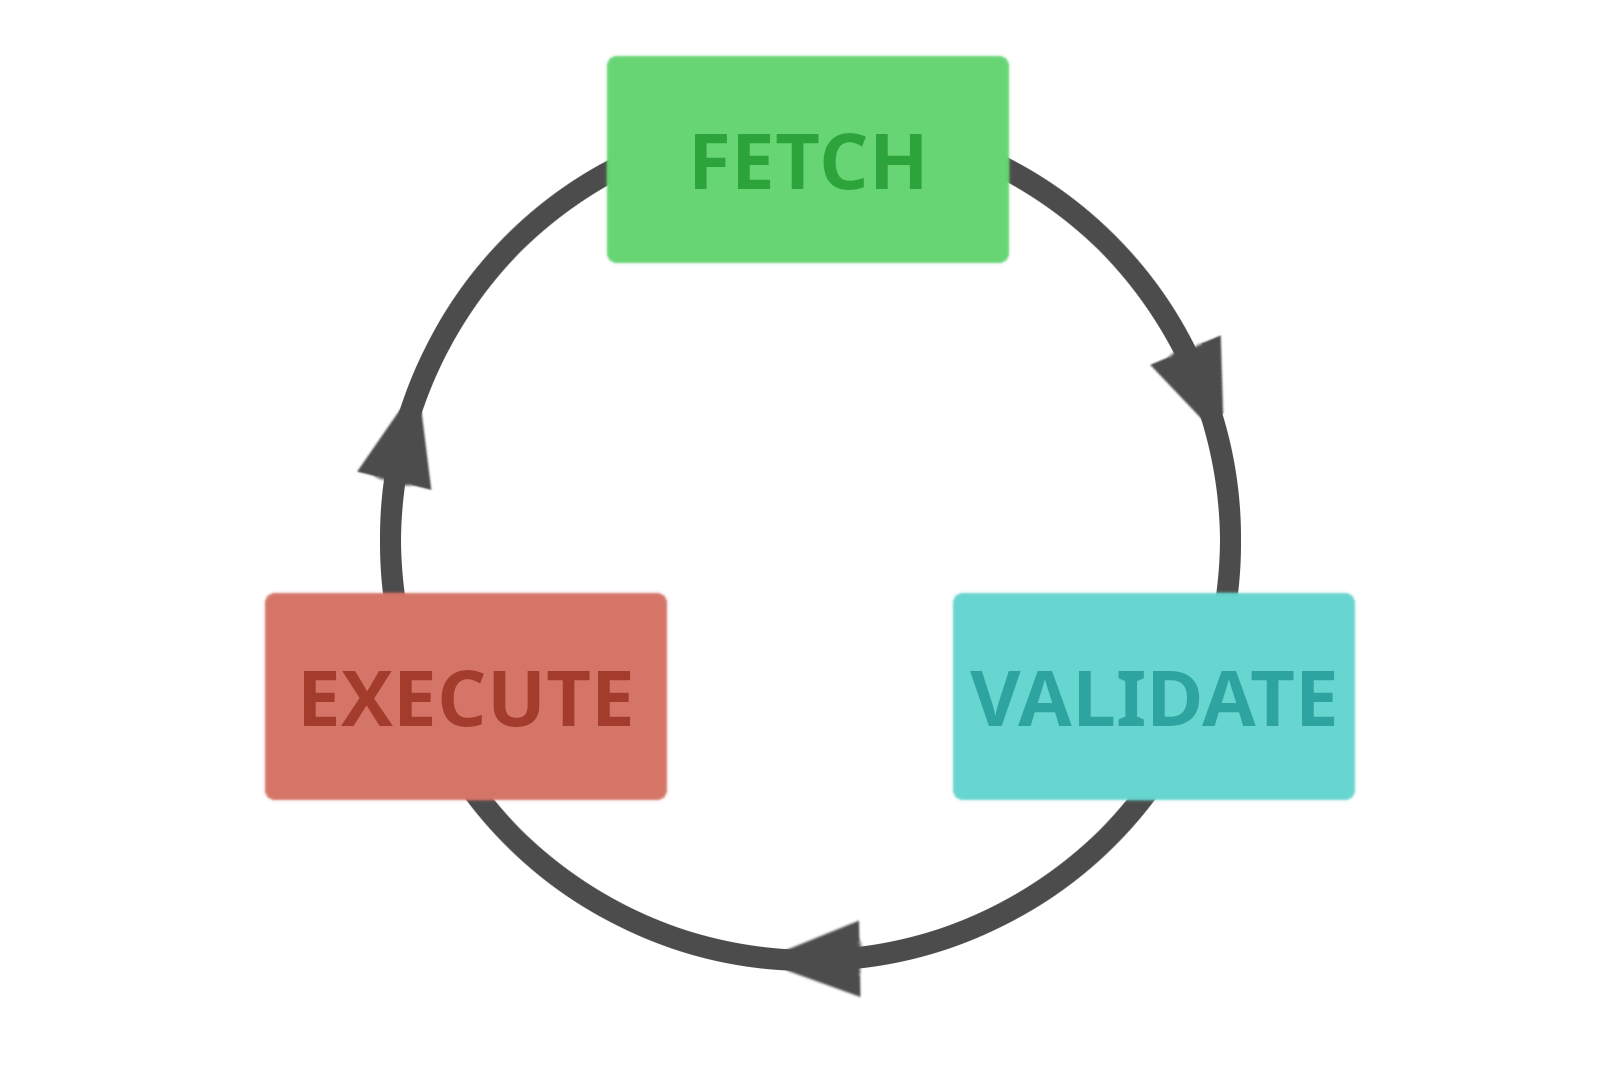
\includegraphics[scale=0.75]{resources/images/qhs-cycle.png}
    \caption{Zyklus der QHS Kompilierung}
    \label{fig:qhs-cycle}
\end{figure}

\section{Die \textit{Fetch-Phase}} \label{sec:qhs-fetch}
Die Aufgabe der \textit{Fetch-Phase} ist es die nächste \textit{Order}, die verarbeitet werden soll, zu finden. In dieser Hinsicht gleicht die \textit{Fetch-Phase} der lexikalischen Analyse eines traditionellen Compilers.
Der QHS-Zyklus beginnt bei der \textit{Fetch-Phase}, dabei wird die erste \textit{Order} aus der Eingabedatei extrahiert. In jeder weiteren \textit{Fetch-Phase} wird die nächste \textit{Order} aus der Eingabedatei geholt.
Die \textit{Fetch-Phase} ist auch dafür zuständig die nächste \textit{Order} einem der drei Typen (\textit{Identifier}, \textit{Instruction} oder \textit{LiteralCode}) zuzuordnen.
Diese \textit{Ordertypen} sind mit folgenden Regular-Expressions definiert. Leerzeichen dienen als Trennung zwischen \textit{Orders} und werden ignoriert.

\begin{table}[h]
    \fontsize{13}{17}\selectfont
    \centering
    \caption{RegEx Definitionen der \textit{Ordertypen}}
    \vspace{3mm} % Adjust the height of the space between caption and tabular
    
    \begin{tabular}{l>{\listingFont\selectfont}l}
    \multicolumn{1}{l|}{identifier}        & {[}\textasciicircum \textbackslash{}s{]}+                         \\ \hline
    \multicolumn{1}{l|}{instruction}       & \#{[}\textasciicircum \textbackslash{}s{]}+                      \\ \hline
    \multicolumn{1}{l|}{literalCode}       & ".*"                                                              \\
    %                                       &                                                                   \\
    %\textless{}identiferChar\textgreater{} & = {[}\textasciicircum{}\# "\textless{}whitespace\textgreater{}{]} \\
    %\textless{}whitespace\textgreater{}    & = SPACE | NEWLINE | TAB
    
    \end{tabular}
\end{table}

Im Vergleich zu traditionellen Compilern fällt auf, dass beim QHScompiler kaum zwischen Zeichen differenziert wird. Während die lexikalische Analyse traditionell zwischen vielen verschiedenen \textit{Tokens} unterscheidet,
sind für den QHScompiler alle Zeichen (mit Ausnahme von {\listingFont\selectfont \#} und {\listingFont\selectfont "{}}) gleichbedeutend.

Normalerweise erhält die \textit{Fetch-Phase} die nächste \textit{Order} aus der Eingabedatei. 
Es ist jedoch möglich, \textit{Orders} der Eingabedatei voranzustellen. Diese \textit{Orders} werden in der \textit{Fetch-Phase} vor der nächsten \textit{Order} der Eingabedatei gefunden.
Dies geschieht mithilfe des \textit{FetchStacks}, auf den \textit{Orders} gelegt werden können.
In der nächsten \textit{Fetch-Phase} wird immer die oberste \textit{Order} des \textit{FetchStacks} geholt und daraufhin vom \textit{FetchStack} entfernt.
Die Eingabedatei befindet sich auf dem untersten Platz des \textit{FetchStacks} und wird somit nur verwendet, wenn der Stack ansonsten komplett leer ist.
Wann und wie \textit{Orders} auf den \textit{FetchStack} gelegt werden, wird im Abschnitt \ref{sec:qhs-execute} erklärt.
Die Kompilierung ist beendet, sobald der \textit{FetchStack} leer ist.

\section{Die \textit{Enqueue-Phase}} \label{sec:qhs-Enqueue}
Nachdem die nächste \textit{Order} in der  \textit{Fetch-Phase} gefunden wurde, wird diese \textit{Order} an die \textit{Enqueue-Phase} weitergegeben. Während der \textit{Enqueue-Phase} kommt die \textit{OrderQueue} ins Spiel.
Dabei handelt es sich, wie der Name schon sagt, um eine Queue von \textit{Orders}.
Die Aufgabe der \textit{OrderQueue} ist das Speichern und spätere Zurückholen von \textit{Orders}.
Die \textit{OrderQueue} kann mit \textit{Instructions}, die im Abschnitt \ref{sec:qhs-execute} weiter ausgeführt werden, aktiviert und deaktiviert werden.
Wenn eine \textit{Order} in die \textit{Enqueue-Phase} gelangt und die \textit{OrderQueue} aktiviert ist, wird diese \textit{Order} der \textit{OrderQueue} hinzugefügt.
Die \textit{Execute-Phase} wird danach übersprungen und der QHS-Zyklus beginnt von neuem bei Fetch.
Die \textit{Order} wurde (ohne die \textit{Execute-Phase} erreicht zu haben) auf der \textit{OrderQueue} gespeichert.
Später ist es mit \textit{Instructions} möglich diese \textit{Order} von der \textit{OrderQueue} zu entfernen und auszuführen.

Bestimmte \textit{Orders} können jedoch \textit{orderQueue-proof}, also immun gegen die \textit{OrderQueue}, gemacht werden.
\textit{Orders}, die \textit{orderQueue-proof} sind, werden an die \textit{Execute-Phase} weitergegeben, auch wenn die \textit{OrderQueue} aktiv ist.
Dieses Prinzip ist zum Beispiel besonders bei der \textit{Instruction}, welche die \textit{OrderQueue} wieder deaktiviert, wichtig.
Da diese \textit{Instruction} ansonsten nicht zur \textit{Execute-Phase} gelänge und somit die \textit{OrderQueue} nie deaktiviert würde.
%Zu beachten ist, dass \textit{LiteralCode} nicht \textit{orderQueue-proof} sein kann.

%MAYBE OrderQueue FIGURE

Ist die \textit{OrderQueue} deaktiviert oder die \textit{Order} \textit{orderQueue-proof}, gelangt diese \textit{Order} zur \textit{Execute-Phase}.

\section{Die \textit{Execute-Phase}} \label{sec:qhs-execute}
Während der \textit{Execute-Phase} wird die Ausgabedatei generiert. Je nach Typ der \textit{Order} (\textit{Identifier}, \textit{Instruction} oder \textit{LiteralCode}) läuft die \textit{Execute-Phase} sehr unterschiedlich ab.
In den folgenden Abschnitten wird der Ablauf der \textit{Execute-Phase} je nach \textit{Ordertyp} erklärt.

\subsection{\textit{Identifier} in der \textit{Execute-Phase}}
\textit{Identifier} stehen für die am Anfang von Kapitel \ref{cha:4-QHS_Compiler} erwähnten Macros.
Die Macros sind für den QHScompiler eine Liste an \textit{Orders}.
\textit{Identifier} lassen sich zu einer Liste an \textit{Orders} definieren.
Wenn nun ein \textit{Identifier} in die \textit{Execute-Phase} gelangt, werden die dazugehörigen \textit{Orders} auf den \textit{FetchStack} aus Abschnitt \ref{sec:qhs-fetch} gelegt.
Bei den nächsten \textit{Fetch-Phasen} werden nun zuerst die zum \textit{Identifier} gehörenden \textit{Orders} nacheinander abgebaut. Einfach ausgedrückt wird der \textit{Identifier} also durch seine \textit{Orders} ersetzt.
Als Beispiel seien folgende \textit{Identifier} definiert:

\begin{table}[H]
    \centering
    \caption{Definition von \textit{Identifiern} als Beispiel}
    \vspace{3mm} % Adjust the height of the space between caption and tabular    
    
    \begin{tabular}{l|l}
    \textbf{Identifier} & \textbf{Definition}   \\ \hline
    \listingFont\selectfont id1 & \listingFont\selectfont "lit1"                                \\ \hline
    \listingFont\selectfont id2 & \listingFont\selectfont \#inst2.1 "lit2" { }\#inst2.2         \\ \hline
    \listingFont\selectfont id3 & \listingFont\selectfont id2 "lit3"     
    \end{tabular}
\end{table}

Mit diesen \textit{Identifiern}, wird nun folgender Code kompiliert:

\begin{lstlisting}[language=QHS, caption=QHS-Code zur Veranschaulichung von \textit{Identifiern}]
%\ruleEingabe%
"lit0.1"
id1
"lit0.2" id2
id3
%\ruleAusgabe%
"lit0.1"
"lit1"
"lit0.2" #inst2.1 "lit2" #inst2.2
#inst2.1 "lit2" #inst2.2 "lit3"
\end{lstlisting}

Die \textit{Identifier} aus der Eingabe wurden mit ihren Definitionen ersetzt. Wie der \textit{Identifier} {\listingFont\selectfont id3} zeigt, ist es möglich \textit{Identifier} ineinander zu verschachteln.

Die Definitionen der \textit{Identifier} sind in einem sogenannten \textit{Environment} definiert.
Bei einem \textit{Environment} handelt es sich um eine einfache Map, die einen \textit{Identifier} mit einer Liste an \textit{Orders} verknüpft.
\textit{Environments} sind in einer verketteten Liste gespeichert. Neue \textit{Environments} können dieser Liste hinzugefügt und aus der Liste entfernt werden.
Das letzte \textit{Environment} der Liste ist das älteste und das erste \textit{Environment} das neuste.
Ein neuer \textit{Identifier} wird immer zum ersten \textit{Environment} der Liste hinzugefügt. Definitionen des gleichen \textit{Identifiers} in älteren \textit{Environments} werden nicht überschrieben oder gelöscht.
Bei der Abfrage nach einem \textit{Identifier} wird immer die neuste vorhandene Definition zurückgegeben.
In Abschnitt \ref{sec:howto-identifiers} werden \textit{Environments} anhand eines Beispiels erneut aufgegriffen.

\subsection{\textit{Instruction} in der \textit{Execute-Phase}}
%\textit{Instructions} sind die komplexesten \textit{Orders} für die \textit{Execute-Phase}. 
Wenn eine \textit{Instruction} in die \textit{Execute-Phase} gelangt, wird die dazu definierte Funktion im QHScompiler ausgeführt.
Diese Funktionen können \textit{Identifier} definieren, die \textit{OrderQueue} aktivieren, Zahlen addieren und vieles mehr.
\textit{Instructions} sind somit der Weg wie während der Kompilierung auf den QHScompiler Einfluss genommen werden kann.
In der Tabelle \ref{tab:important_instructions} sind \textit{Instructions} aufgelistet, die in späteren Beispielen verwendet werden.

\begin{table}[H]
    \centering
    \caption{Wichtige Instructions des QHScompilers}
    \label{tab:important_instructions}
    \vspace{3mm} % Adjust the height of the space between caption and tabular
    
    \begin{tabularx}{\textwidth}{l|X}
    \textbf{Instruction}                             & \textbf{Beschreibung} \\ \hline
    {\listingFont\selectfont \#enterOrderQueue}      & Aktiviert die \textit{OrderQueue}. Diese \textit{Instruction} ist \textit{orderQueue-proof}. \\ \hline
    {\listingFont\selectfont \#exitOrderQueue}       & Deaktiviert die \textit{OrderQueue}. Diese \textit{Instruction} ist \textit{orderQueue-proof}. \\ \hline
    {\listingFont\selectfont \#assign}               & Die erste \textit{Order} der \textit{OrderQueue} muss ein \textit{Identifier} sein.
                                                       Der Rest der \textit{Orders} auf der \textit{OrderQueue} wird als Definition für diesen \textit{Identifier} festgelegt. \\ \hline
    {\listingFont\selectfont \#assignToOne}          & Wie {\listingFont\selectfont \#assign}, jedoch wird nach dem \textit{Identifier} nur eine weitere \textit{Order} von der \textit{OrderQueue} genommen und 
                                                       als Definition für den \textit{Identifier} verwendet. \\ \hline
    {\listingFont\selectfont \#force}                & Die nächste \textit{Order} wird nach der \textit{Fetch-Phase} sofort an die \textit{Execute-Phase} weitergegeben.
                                                       Überspringt die \textit{Enqueue-Phase} und somit die \textit{OrderQueue}. Diese \textit{Instruction} ist \textit{orderQueue-proof}. \\ \hline
    %{\listingFont\selectfont \#lightForce}           & Ähnlich wird {\listingFont\selectfont \#force}, jedoch wird diese nur ausgeführt, wenn \textbf{explain this cuz they don't know OrderQueue depth} \\ \hline
    {\listingFont\selectfont \#orderEnqueue}         & Die nächste \textit{Order} wird sofort dem Ende der \textit{OrderQueue} hinzugefügt, auch wenn diese \textit{Order} \textit{orderQueue-proof} wäre.
                                                       Die \textit{Execute-Phase} wird übersprungen. \\ \hline
    {\listingFont\selectfont \#orderFrontEnqueue}    & Ähnlich wie {\listingFont\selectfont \#orderEnqueue}. Die \textit{Order} wird jedoch an den ersten Platz der \textit{OrderQueue} gesetzt. \\ \hline
    {\listingFont\selectfont \#deepFetch}            & Die nächste \textit{Order} der Eingabedatei wird oben auf den \textit{FetchStack} gesetzt. Ermöglicht den Zugriff auf die Eingabedatei innerhalb eines \textit{Identifiers}. \\ \hline
    {\listingFont\selectfont \#queueFetch}           & Die erste \textit{Order} der \textit{OrderQueue} wird oben auf den \textit{FetchStack} gesetzt. \\ \hline 
    {\listingFont\selectfont \#pushEnv}              & Ein neues \textit{Environment} wird der \textit{Environment-Liste} hinzugefügt. \\ \hline
    {\listingFont\selectfont \#popEnv}               & Das neuste \textit{Environment} der \textit{Environment-Liste} wird gelöscht. \\ \hline
    {\listingFont\selectfont \#addToIdentifier}      & Die erste \textit{Order} der \textit{OrderQueue} muss ein \textit{Identifier} sein und die zweite \textit{LiteralCode}. Die Definition des \textit{Identifiers} muss eine Zahl sein.
                                                       Der \textit{LiteralCode} wird zu dieser Zahl addiert und im \textit{Identifier} gespeichert.       
    \end{tabularx}
\end{table}

Der QHScompiler umfasst 31 \textit{Instructions}, wobei 5 dieser ausschliesslich fürs Debuggen des Compilers dienen.

\subsection{\textit{LiteralCode} in der \textit{Execute-Phase}}
\textit{LiteralCode} ist der Weg wie der QHScompiler Assembly-Code generiert. Dieser ist sehr einfach.
Wenn \textit{LiteralCode} in die \textit{Execute-Phase} gelangt, wird alles, das zwischen den Satzzeichen steht, in die Ausgabedatei geschrieben.
Dies ist die einzige Möglichkeit des QHScompiler Assembly-Code zu generieren. Einzig die \textit{LiteralCode-Orders} bestimmen, was in die Ausgabedatei gelangt, und somit welcher Sprache diese Ausgabedatei folgt. 
Durch das Anpassen der \textit{LiteralCode-Orders} ist es also möglich die Ausgabesprache des QHScompilers zu ändern.


\section{Definition der Macros} \label{sec:qhs-macro_definitions}
Somit ist der QHScompiler komplett. Grundsätzlich lässt sich mit \textit{LiteralCode} bereits jedes Programm schreiben und mit dem QHScompiler kompilieren. 
Jedoch muss, wie in Kapitel \ref{cha:2-Vergleich} festgelegt, ie Eingabesprache eine C-ähnliche Syntax aufweisen und die Ausgabesprache Assembly sein.
Um dies zu ermöglichen, muss man, wie zu Beginn von Kapitel \ref{cha:4-QHS_Compiler} erwähnt, bestimmte Macros, also \textit{Identifier}, definieren.
In diesem Abschnitt werde ich zeigen, wie sich diese \textit{Identifier} auch für syntaktisch komplexe Programmiersprachen definieren lassen.
Zur Veranschaulichung dienen Variablen und Funktionsdefinitionen.


\iffalse
Der QHScompiler ist zwar komplett, die dazugehörige Programmiersprache QHS jedoch noch lange nicht.
Grundsätzlich ist es möglich mit \textit{LiteralCode} jedes Programm zu schreiben und zu kompilieren, jedoch handelt es sich dann nur um Assembly-Code.
Doch der Aufbau des QHScompilers ermöglicht es mit \textit{Identifiern} eine komplexere Programmiersprache zu definieren. Ein fester Bestandteil ein jedes Programms, das mit dem QHScompiler kompiliert werden soll, ist ein Stück Code,
das die jeweilige Programmiersprache definiert. Dieser Code wird im Kontext des QHScompilers \textit{Preamble} genannt. Theoretisch ist es möglich durch das Anpassen dieses Preambles, 
viele unterschiedliche Programmiersprachen mit dem QHScompiler zu kompilieren. In diesem Abschnitt wird behandelt wie sich die Sprache QHS, welche die Kriterien aus Abschnitt \ref{sec:Vergleichs_Kriterien} erfüllt,
für den QHScompiler definieren lässt.
\fi

\subsection{Die QHS-Notation} \label{sec:qhs-notation}
In diesem Abschnitt wird viel QHS-Code als Beispiel verwendet.
Um die Leserlichkeit von QHS zu verbessern, werden zuerst paar \textit{Identifier} anstelle der umständlichen \textit{Instructions} definiert.
Diese \textit{Identifier} sind in der folgenden Tabelle \ref{tab:shortcuts} aufgeführt.

{
\begin{table}[H]
    \centering
    \caption{\textit{Identifier} als Abkürzung von \textit{Instructions}}
    \vspace{3mm} % Adjust the height of the space between caption and tabular
    \label{tab:shortcuts}
    
    \begin{tabular}{l|l}
    \textbf{Identifier}                                     & \textbf{Definition}            \\ \hline
    {\listingFont\selectfont [}                             & {\listingFont\selectfont \#enterOrderQueue}              \\ \hline
    {\listingFont\selectfont ]}                             & {\listingFont\selectfont \#exitOrderQueue}               \\ \hline
    {\listingFont\selectfont \textgreater{}\textgreater{}}  & {\listingFont\selectfont \#assign}                       \\ \hline
    {\listingFont\selectfont -\textgreater{}}               & {\listingFont\selectfont \#assignToOne}                  \\ \hline
    {\listingFont\selectfont !}                             & {\listingFont\selectfont \#force}                        \\ \hline
    %{\listingFont\selectfont ?!}                            & {\listingFont\selectfont \#lightForce}                   \\ \hline
    {\listingFont\selectfont \textbackslash{}n}             & Eine neue Zeile in der Ausgabedatei                      \\ \hline
    {\listingFont\selectfont /*}                            & Beginn eines Kommentars                                  \\ \hline
    {\listingFont\selectfont */}                            & Ende eines Kommentars
    \end{tabular}
\end{table}
}

Innerhalb von Kommentaren wird Pseudo-Code verwendet, um den QHS-Code verständlicher zu erklären.
Kommentare können mehrere Zeilen umfassen und beginnen immer mit {\listingFont\selectfont /*} und enden mit {\listingFont\selectfont*/}.
Der Kommentar {\listingFont\selectfont /* X = "test" { }\#pushEnv */} würde bedeuten,
dass der \textit{Identifier} {\listingFont\selectfont X} als Folge der \textit{Orders} {\listingFont\selectfont "test"{}} (\textit{LiteralCode}) und {\listingFont\selectfont \#pushEnv} (\textit{Instruction}) definiert wurde. 

%Auch wird bei längeren \textit{Identifier}-Definitionen zuerst der zu definierende \textit{Identifier} getrennt von den restlichen \textit{Orders} der \textit{OrderQueue} hinzugefügt.
%Diese Separation dient der besseren Leserlichkeit und hat keinen Einfluss auf die Kompilierung des Codes.

\subsection{Beispiele zu \textit{Identifier}-Definitionen} \label{sec:howto-identifiers}
Wie die Definition von \textit{Identifiern} ablaufen kann, wird in diesem Abschnitt an einigen Beispielen erklärt.

\begin{minipage}{\linewidth}
\begin{multicols}{2}
\begin{lstlisting}[language=QHS, label=eg:howto_id1-3, caption=Beispiel zu gewöhnlichen \textit{Identifier}-Definitionen, numbers=left, stepnumber=1]
%\ruleEingabe%
[ id1 "lit1" ] ->
[ id2 "lit2.1" "lit2.2" id1 ] >>
[ id3 ] [ "lit3.1" "lit3.2" ] >>

id1 \n
id2 \n
id3

%\ruleAusgabe%

lit1
lit2.1 lit2.2 lit1
lit3.1 lit3.2
\end{lstlisting}
\columnbreak
\iffalse
    In Linie 1 wird zuerst die \textit{OrderQueue} geöffnet und die Orders {\selectListingFont id1} und {\selectListingFont "lit1"{}} hinzugefügt.
    Schliessen sieht die \textit{OrderQueue} wie folgt aus:
    \centerline{\selectListingFont id1 "lit1"{}}
    Mit {\selectListingFont ->} wird die erste \textit{Order} der \textit{OrderQueue} ({\selectListingFont id1}) zu der zweiten \textit{Order} ({\selectListingFont "lit1"{}}) definiert.
    \break
    In Linie 2 kommt {\selectListingFont id2}, {\selectListingFont "lit2"{}}, {\selectListingFont \#inst2} und {\selectListingFont id1} auf die \textit{OrderQueue}. Diese sieht daraufhin wie folgt aus:
    \centerline{\selectListingFont id2 "lit2"{} \#inst2 id1}
    Der Identifier {\selectListingFont >>} definiert die erste \textit{Order} der \textit{OrderQueue} ({\selectListingFont id2}) zu allen restlichen \textit{Order} auf der \textit{OrderQueue}.
    Die Definition von {\selectListingFont id2} ist daraufhin:
    \centerline{\selectListingFont id2 = "lit2"{} \#inst2 id1}
\fi
Die Linien 2 und 3 definieren die folgenden beiden \textit{Identifier}: \break
\centerline{\selectListingFont id1 = "lit1"{}}
\centerline{\selectListingFont id2 = "lit2.1"{} "lit2.2"{} id1}
In Linie 4 wird die \textit{OrderQueue} zwischendurch deaktiviert und wieder aktiviert.
Dies hat keinen Einfluss auf die Kompilierung und wird daher für die Verbesserung der Leserlichkeit von langen \textit{Identifier}-Definitionen verwendet.
Die \textit{OrderQueue} sieht vor dem {\selectListingFont >>} wie folgt aus, wobei das linkste Element das erste darstellt:  \break
\centerline{\selectListingFont id3 "lit3.1"{} "lit3.2"{}}
Wie gewohnt wird {\selectListingFont id3} mit {\selectListingFont >>} definiert: \break
\centerline{\selectListingFont id3 = "lit3.1"{} "lit3.2"{}}
\end{multicols}
\end{minipage}
\vspace{\baselineskip}

\begin{minipage}{\linewidth}
\begin{multicols}{2}
\begin{lstlisting}[language=QHS, caption=Beispiel zu {\selectListingFont \#assignToOne}, numbers=left, stepnumber=1]
%\ruleEingabe%
[ id4 "lit4" ] >>
[ id5 "lit5" id6 ] ->
[ "lit6" ] >>

id4 \n
id5 \n
id6



%\ruleAusgabe%

lit4
lit5
lit6
\end{lstlisting}
\columnbreak
Die Definition von {\selectListingFont id4} ist hier ähnlich wie in Linie 2 der Auflistung \ref{eg:howto_id1-3}.
Jedoch wird hier anstelle von {\selectListingFont ->} ({\selectListingFont \#assignToOne}) der \textit{Identifier} {\selectListingFont >>} ({\selectListingFont \#assign}) verwendet.
Da sich in beiden Fällen jedoch nur eine weitere \textit{Order} neben dem \textit{Identifier} auf der \textit{OrderQueue} befinden, macht die Verwendung von {\selectListingFont >>} keinen Unterschied.
Bei Linie 3 und 4 ist dies jedoch anders. Zuerst werden drei \textit{Orders} auf die \textit{OrderQueue} gelegt. Der \textit{Identifier} {\selectListingFont ->} definiert daraufhin {\selectListingFont id5} wie folgt: \break
\centerline{\selectListingFont id5 = "lit5"{}}
Der \textit{Identifier} {\selectListingFont id6} bleibt auf der \textit{OrderQueue}.
Erst nachdem {\selectListingFont "lit6"{}} der \textit{OrderQueue} hinzugefügt wurde, wird {\selectListingFont id6} durch {\selectListingFont >>} definiert: \break
\centerline{\selectListingFont id6 = "lit6"{}}
\end{multicols}
\end{minipage}
\vspace{\baselineskip}

\begin{minipage}{\linewidth}
\begin{multicols}{2}
\begin{lstlisting}[language=QHS, caption=Beispiel zu {\selectListingFont \#orderFrontEnqueue}, numbers=left, stepnumber=1]
%\ruleEingabe%
[ "lit7.1" ]
#orderFrontEnqueue id7
[ "lit7.2" ] >>

id7



%\ruleAusgabe%

lit7.1 lit7.2
\end{lstlisting}
\columnbreak
Zuerst gelangt {\selectListingFont "lit7.1"{}} auf die \textit{OrderQueue}.
Daraufhin wird mit der \textit{Instruction} {\selectListingFont \#orderFrontEnqueue} der \textit{Identifier} {\selectListingFont id7} auf die erste Position der \textit{OrderQueue} gesetzt.
Die \textit{OrderQueue} sieht daraufhin wie folgt aus:
\centerline{\selectListingFont id7 "lit7.1"{}}
Der \textit{LiteralCode} {\selectListingFont "lit7.2"{}} wird normal hinten an die \textit{OrderQueue} angefügt.
Da sich der Identifer {\selectListingFont id7} auf dem ersten Platz der \textit{OrderQueue} befinden, kann dieser definiert werden: \break
\centerline{\selectListingFont id7 = "lit7.1"{} "lit7.2"{}}
\end{multicols}
\end{minipage}
\vspace{\baselineskip}

\begin{minipage}{\linewidth}
\begin{multicols}{2}
\begin{lstlisting}[language=QHS, label=eg:howto-id8, caption=Beispiel zu doppelter Aktivierung der \textit{OrderQueue}, numbers=left, stepnumber=1]
%\ruleEingabe%
[ id8 ]
[
    "lit8.1"
    [ "lit8.2" ]
] >>

id8



%\ruleAusgabe%

lit8.1
Die OrderQueue enthält: "lit8.2"
\end{lstlisting}
\columnbreak
In Auflistung \ref{eg:howto-id8} wird eine \textit{Identifier}-Definition auf mehrere Zeilen aufgeteilt. Dies dient der besseren Leserlichkeit und kompiliert gleich wie eine Definition auf nur einer Linie.
Auf Linie 5 werden {\selectListingFont [} ({\selectListingFont \#enterOrderQueue}) und {\selectListingFont ]} ({\selectListingFont \#exitOrderQueue}) innerhalb einer bereits aktiven \textit{OrderQueue} verwendet.
Im QHScompiler ist dies so implementiert, dass die beiden \textit{Identifier} nicht ausgeführt und normal der \textit{OrderQueue} hinzugefügt werden. Die \textit{OrderQueue} enthält nach Linie 5 folgende \textit{Orders}: \break
\centerline{\selectListingFont id8 "lit8.1"{} [ "lit8.2"{} ] }
Die \textit{Identifier} {\selectListingFont [} und {\selectListingFont ]} gelangen normal in die \textit{OrderQueue} und damit auch in die Definition von {\selectListingFont id8}: \break
\centerline{\selectListingFont id8 = "lit8.1"{} [ "lit8.2"{} ] }
\end{multicols}
\end{minipage}
\vspace{\baselineskip}

\begin{minipage}{\linewidth}
\begin{multicols}{2}
\begin{lstlisting}[language=QHS, label=eg:howto-id9, caption=Beispiel zu {\selectListingFont \#force} , numbers=left, stepnumber=1]
%\ruleEingabe%
[ id9 "lit9" ] >>

[ id10 ]
[
    ! id9
    [ ! id9 ]
] >>

id9  \n
id10




%\ruleAusgabe%

lit9
lit9
Die OrderQueue enthält: "lit9"
\end{lstlisting}
\columnbreak
Zuerst wird in Linie 2 der \textit{Identifier} {\selectListingFont id9} wie gewohnt definiert. In Linie 6 wird der \textit{Identifier} {\selectListingFont !} ({\selectListingFont \#force}) verwendet.
Die \textit{Instruction} {\selectListingFont \#force} ist \textit{orderQueue-proof} und zwingt den QHScompiler dazu, die nächste \textit{Order} an die \textit{Execute-Phase} weiterzugeben, obwohl die \textit{OrderQueue} aktiv ist.
Der \textit{Identifier} {\selectListingFont id9} wird daher mit seiner Definition ersetzt. Die \textit{OrderQueue} sieht nach Linie 6 wie folgt aus: \break
\centerline{\selectListingFont id10 "lit9"{}}
In Linie 7 wird daraufhin der \textit{Identifer} {\selectListingFont !} erneut verwendet. Dieses Mal jedoch innerhalb einer doppelten Aktivierung der \textit{OrderQueue}, wie in Beispiel \ref{eg:howto-id8}.
In diesem Fall gelangen auch \textit{Orders} die \textit{orderQueue-proof} sind, nicht zur \textit{Execute-Phase}. Der \textit{Identifier} {\selectListingFont !} wird normal der \textit{OrderQueue} hinzugefügt.
Die folgende Definition von {\selectListingFont id10} lautet: \break
\centerline{\selectListingFont id10 = "lit9"{} [ ! id9 ]}
\end{multicols}
\end{minipage}
\vspace{\baselineskip}

\begin{minipage}{\linewidth}
\begin{multicols}{2}
\begin{lstlisting}[language=QHS, caption=Beispiel zu \textit{Environments}, numbers=left, stepnumber=1]
%\ruleEingabe%
[ id11 "lit11.1" ] >>
[ id12 "lit12" ] >>

id11 " " id12 \n

#pushEnv

[ id11 "lit11.2" ] >>
id11 " " id12 \n

#popEnv

id11 " " id12
%\ruleAusgabe%
lit11.1 lit12
lit11.2 lit12
lit11.1 lit12
\end{lstlisting}
\columnbreak
Die \textit{Identifier} {\selectListingFont id11} und {\selectListingFont id12} werden gewöhnlich definiert und verwendet. Daraufhin wird mit {\selectListingFont \#pushEnv} ein neues \textit{Environment} hinzugefügt.
In diesem \textit{Environment} wird {\selectListingFont id11} umdefiniert. In Linie 12 wird die neuste Definition der beiden \textit{Identifier} verwendet. Für {\selectListingFont id11} ist dies: \break
\centerline{\selectListingFont id11 = "lit11.2"}
Der Definition des {\selectListingFont id12} \textit{Identifiers} ist unverändert: \break
\centerline{\selectListingFont id12 = "lit12"}
Mit der \textit{Instruction} {\selectListingFont \#popEnv} wird das neuste \textit{Environment} gelöscht und die geänderte Definition von {\selectListingFont id11} vergessen.
Die Definition vom \textit{Identifier} {\selectListingFont id11} ist wieder:
\centerline{\selectListingFont id11 = "lit11.1"}
\end{multicols}
\end{minipage}



\subsection{Parameter und Rückgabewert für \textit{Identifier}}
Mit den {\listingFont\selectfont \#enterOrderQueue} (resp. {\listingFont\selectfont [} ) und {\listingFont\selectfont \#exitOrderQueue} (resp. {\listingFont\selectfont ]} ) \textit{Instructions}
kann innerhalb eines \textit{Identifiers} die \textit{OrderQueue} verwendet werden.
Dies ermöglicht eine Art von Parameter und Rückgabewert für \textit{Identifier}.
Vor dem Aufruf eines \textit{Identifiers} lassen sich \textit{Orders} der \textit{OrderQueue} hinzugefügen. Diese \textit{Orders} können dann innerhalb des \textit{Identifiers} wie Parameter verwendet werden.
Genauso kann der \textit{Identifier} \textit{Orders} der \textit{OrderQueue} hinzufügen und diese somit zurückgeben.

\begin{lstlisting}[language=QHS, caption=Verwendung von Parametern und Rückgabewert eines \textit{Identifiers}]
%\ruleEingabe%
[ foo ]
[
    #orderFrontEnqueue param1 ->    /* param1 = erstes Argument */
    #orderFrontEnqueue param2 ->    /* param2 = zweites Argument */

    param1 " : " param2 \n          /* param1 + " : " + param2 + "\n" */

    [ "Rückgabewert" ]              /* "Rückgabewert" wird der OrderQueue hinzugefügt */
] >>

[ "Argument 1" "Argument 2" ]       /* 2 Argumente werden der OrderQueue hinzugefügt */
foo                                 /* foo wird ausgeführt */
#queueFetch                         /* Die zurückgegebene Order wird von der OrderQueue
                                    geholt und ausgeführt */


%\ruleAusgabe%
Argument 1 : Argument 2
Rückgabewert
\end{lstlisting}


\subsection{Variablen} \label{sec:qhs-vars}
Nun da die Grundkonzepte von QHS erklärt sind, geht es darum \textit{Identifier} für einen C ähnlichen Syntax zu definieren.
Die Umsetzung von Variablen in QHS ist einfach.
Um Platz für die Variable auf dem Stack zu schaffen, muss zuerst die Grösse der Variable (für dieses Beispiel vier Bytes) vom \textit{Stack-Pointer} subtrahiert werden.
Dann wird für die Variable ein \textit{Identifier} definiert, der zur Position der Variable auf dem Stack zeigt.
Mit \textit{LiteralCode} lässt sich dies wie folgt in QHS ausdrücken:

\begin{lstlisting}[language=QHS, caption=Definition einer Variable mit \textit{LiteralCode}]
%\ruleEingabe%
"sub rsp, 4" \n
[ a "[rbp-4]" ] >>      /* a = "[rbp-4]" */

"add " a ", 5"

%\ruleAusgabe%
sub rsp, 4
add [rbp-4], 5
\end{lstlisting}

Jedoch braucht man für diese Implementation immer noch Assembly Kenntnisse.
Um die Definition von Variablen C ähnlicher zu machen, lässt sich zum Beispiel ein {\selectListingFont var} \textit{Identifier} definieren.
Dieser {\selectListingFont var} \textit{Identifier} nimmt die Grösse der Variable als Argument über die \textit{OrderQueue} an. Um die in C geläufige Syntax der Definition einer Variable beizubehalten,
wird der Name der Variable mit der {\listingFont\selectfont \#deepFetch} \textit{Instruction} beschafft.

\begin{lstlisting}[language=QHS, caption=Definition einer Variable mit {\selectListingFont var} \textit{Identifier}]
%\ruleEingabe%
[ var ]
[
    #orderFrontEnqueue size ->          /* size = erstes Argument */
    [ name ! #deepFetch ] >>            /* name = Was nach dem var Identifer folgt */

    "sub rsp, " size \n

    [ ! name ] [ "[rbp-4]" ] >>             /* Was name enthält = "[rbp-4]" */
] >> 

[ "4" ] var a 
[ "8" ] var b 

"add " a ", 5"
"sub " b ", 10"
    
%\ruleAusgabe%
sub rsp, 4
sub rsp, 8
add [rbp-4], 5
sub [rbp-4], 10
\end{lstlisting}

Momentan erhält jede Variable jedoch noch die Adresse {\selectListingFont rbp-4}, weswegen sich die Variablen gegenseitig überschreiben würden. Der momentane Abstand zum Base-Pointer muss also gespeichert und erhöht werden.
Dafür wird bereits am Anfang des Programms ein \textit{Identifier} {\selectListingFont rbpOffset} als 0 definiert.
Mit der {\listingFont\selectfont \#addToIdentifier} \textit{Instruction}, lässt sich nun {\selectListingFont rbpOffset} erhöhen. Dies kann folgendermassen aussehen:

\begin{minipage}{\linewidth}
\begin{lstlisting}[language=QHS, label=eg:qhs-vardefinition, caption=Definition einer Variable mit rbpOffset]
%\ruleEingabe%
[ rbpOffset "0" ] >>                    /* rbpOffset = "0" */

[ var ]
[
    #orderFrontEnqueue size ->          /* size = erstes Argument */
    [ name ! #deepFetch ] >>            /* name = Was nach dem var Identifier folgt */

    "sub rsp, " size \n

    [ rbpOffset ! size ] #addToIdentifier      /* rbpOffset += size */

    [ ! name ] [ "[rbp-" ! rbpOffset "]" ] >>  /* Was name enthält = "[rbp-OFFSET]" */
] >> 

[ "4" ] var a 
[ "8" ] var b 

"add " a ", 5"
"sub " b ", 10"
    
%\ruleAusgabe%
sub rsp, 4
sub rsp, 8
add [rbp-4], 5
sub [rbp-12], 10
\end{lstlisting}
\end{minipage}

Zuletzt lässt sich das umständliche Hinzufügen der Grösse der Variable sowie der {\selectListingFont var} \textit{Identifier} unter einem neuen \textit{Identifier} zusammenfassen.
Dies ist passenderweise die bekannte Bezeichnung für den Typen der Variable.

\begin{lstlisting}[language=QHS, caption=Definition einer Variable mit {\selectListingFont int} \textit{Identifier}]
%\ruleEingabe%
(...)

[ int ] 
[
    [ "4" ] var
] >>
    
int a 
int b 
    
"add " a ", 5"
"sub " b ", 10"
        
%\ruleAusgabe%
sub rsp, 4
sub rsp, 8
add [rbp-4], 5
sub [rbp-12], 10
\end{lstlisting}

Nun sieht die Definition und Verwendung einer Variable genau so aus, wie es in C gebräuchlich ist.
Auf das Setzten von Variablen werde ich hier nicht weiter eingehen, da dies mit den Methoden, die im nächsten Abschnitt \ref{sec:qhs-funcs} erklärt werden, funktioniert.

\subsection{Funktionsdefinitionen} \label{sec:qhs-funcs}
Funktionen sind im Vergleich zu Variablen komplizierter. Nachfolgend sollen zwei der Probleme von Funktionsdefinitionen behandelt werden.
Anhand einer Funktionsdefinition, wie sie zum Schluss aussehen sollte, will ich die beiden Probleme erläutern:

\begin{lstlisting}[language=C, label=eg:qhs-function_goal, caption=Ziel für die Definition einer Funktion in QHS]
int foo ( int param1 , int param2 )
{
    (...)
}
\end{lstlisting}

Hier lässt sich bereits das erste Problem feststellen. Im vorherigen Abschnitt \ref{sec:qhs-vars} wurde der {\selectListingFont int} \textit{Identifier} für die Definition einer Variable verwendet. 
Das {\selectListingFont int} in der Auflistung \ref{eg:qhs-function_goal} würde daher vom QHScompiler als Definition für eine Variable verstanden werden.
Der Unterschied zwischen Variablen- und Funktionsdefinition besteht hierbei in den Klammern, die auf den Namen folgen.
Der QHScompiler müsste also beim {\selectListingFont int} \textit{Identifier} nach vorne schauen, ob sich eine Klammer nach dem Namen befindet, und folglich eine Variablen- oder Funktionsdefinition ausführen.
Bei einem traditionellen Compiler würde diese Überprüfung während der syntaktischen Analyse ausgeführt werden.
Dies ist dem QHScompiler jedoch nicht möglich, da dieser, wie zu Beginn von Kapitel \ref{cha:4-QHS_Compiler} erläutert, über keine syntaktische Analyse verfügt.
Glücklicherweise lässt sich dieses erste Problem lösen, ohne eine Änderung am QHScompiler vorzunehmen.
Die Lösung basiert darauf, beim {\selectListingFont int} \textit{Identifier} sowohl eine Variablen- als auch eine Funktionsdefinition vorzubereiten, aber keine der beiden bereits auszuführen.
Daraufhin werden zwei \textit{Identifier} definiert, erstens eine Klammer für eine Funktionsdefinition und zweitens ein Semikolon für die Definition einer Variable.
%Daraufhin wird eine Klammer als \textit{Identifier} für eine Funktionsdefinition und ein Semikolon für die Definition einer Variable definiert.
Befindet sich nach dem Namen eine Klammer, wird eine Funktionsdefinition ausgeführt, ist dort aber ein Semikolon wird eine Variable definiert.
Dieses Konzept wird im weiteren als \textit{DelayedExecute} bezeichnet. Das Ganze sieht danach wie folgt aus:

%minipage keeps the listing from splitting onto multiple pages
\begin{minipage}{\linewidth}
\begin{lstlisting}[language=QHS, caption=Implementation eines \textit{DelayedExecute} für Definitionen]
(Definition einer Variable aus Auflistung %\ref{eg:qhs-vardefinition}%)

[ function ]
[
    #orderFrontEnqueue returnSize ->        /* size = erstes Argument */
    #orderFrontEnqueue name ->              /* name = zweites Argument */

    [ ! name ] #orderToLiteral ":" \n       /* "foo:" */
] >>

[ definition ]
[
    #orderFrontEnqueue size ->           /* size = erstes Argument */
    [ name ! #deepFetch ] >>             /* name = Was nach dem var Identifier folgt */

    [ ; ]
    [
        [ ! size ! name ] var 
    ] >>
    /* ; = [ size name ] var */

    [ ( ]
    [
        [ ! size ! name ] function 
    ] >>
    /* ( = [ size name ] function */

] >>

[ int ]
[
    [ "4" ] definition
] >>
\end{lstlisting}
\end{minipage}


Das zweite Problem sind die Parameter einer Funktionsdefinition. Diese sehen genau gleich aus wie die Definition einer Variable, sollten jedoch vom QHScompiler anders ausgeführt werden.
Erstens wird bei der Definition von Variablen aus Abschnitt \ref{sec:qhs-vars} \textit{LiteralCode} zur Subtraktion vom \textit{Stack-Pointer} verwendet. Diese Subtraktion braucht es bei Parameterdefinition nicht.
%Erstens sollte bei einer Parameterdefinition nicht der \textit{LiteralCode} zur Subtraktion vom \textit{Stack-Pointer}, wie bei Definition von Variablen aus Abschnitt \ref{sec:qhs-vars}, hinzugefügt werden.
Zweitens verwendet eine Parameterdefinition einen anderen rbp-Offset als Definitionen von Variablen.
Die Lösung liegt im Umdefinieren des {\selectListingFont definition} \textit{Identifiers}. Dieser ist momentan für die Definition von Variablen und Funktionen verantwortlich.
Bei der Anfangsklammer der Funktionsdefinition wird der {\selectListingFont definition} \textit{Identifier} neu definiert, sodass er eine Parameterdefinition ausführt.
Die vorherige Definition geht dank der {\listingFont\selectfont \#pushEnv} \textit{Instruction} nicht verloren.
Bei der schliessenden Klammer wird {\listingFont\selectfont \#popEnv} durchgeführt, und der {\selectListingFont definition} \textit{Identifier} ist wieder für Variablen und Funktionen zuständig.
Diese Lösung wird im folgenden \textit{TempAssign} genannt.
Dies lässt sich in QHS wie folgt umsetzen:

\begin{minipage}{\linewidth}
\begin{lstlisting}[language=QHS, caption=Implementation eines \textit{TempAssigns} für Parameter Definitionen]
[ function ]
[
    #pushEnv

    #orderFrontEnqueue returnSize ->        /* size = erstes Argument */
    #orderFrontEnqueue name ->              /* name = zweites Argument */

    [ ! name ] #orderToLiteral ":" \n       /* "foo:" */

    [ definition paramDefinition ]          /* definition = paramDefinition */
    
    [ ) ] [ #popEnv ] >>                    /* ) = #popEnv */
] >>
\end{lstlisting}
\end{minipage}

Der \textit{Identifier} {\selectListingFont paramDefinition} ist ähnlich wie der {\selectListingFont var} \textit{Identifier} aus Abschnitt \ref{sec:qhs-vars}.
Es wird bloss anstelle von {\selectListingFont rbpOffset} ein neuer {\selectListingFont paramOffset} \textit{Identifier} verwendet und der Assembly-Code fürs Subtrahieren vom \textit{Stack-Pointer} nicht hinzugefügt.

Nun fehlt nur noch etwas an der Funktionsdefinition: Der Funktionsbody. Dieser ist vergleichsweise einfach. Die beiden geschwungenen Klammern werden zu einem leeren \textit{Identifier} definiert und somit ignoriert.
Der gesamte Code innerhalb des Body wird ganz normal vom QHScompiler ausgeführt und an die Ausgabedatei angehängt. Das Endresultat sieht wie folgt aus:

\begin{lstlisting}[language=QHS, caption=Finale Definition einer Funktion in QHS]
%\ruleEingabe%
int foo ( int param1 , int param2 )
{
    "add " param1 ", " param2
}

%\ruleAusgabe%
foo:
add [rbp+16], [rbp+20]
\end{lstlisting}

Wie das Beispiel der Funktionsdefinition zeigt lassen sich mit \textit{DelayedExecute} und \textit{TempAssign} auch syntaktisch komplexe Programmiersprachen in QHS definieren und mit dem QHScompiler kompilieren.

Um einen C ähnlichen Syntax zu ermöglichen, braucht der QHScompiler noch viele weitere \textit{Identifier}.
%Natürlich weist QHS noch viele weitere \textit{Identifier}, die einen C-like Syntax ermöglichen, auf.
Da diese jedoch einem ähnlichen Prinzip wie die beschriebenen Definitionen von Variablen und Funktionen folgen, werde ich sie hier nicht weiter betrachten.


    






